% ------------------------------------------------------------------------------
% TYPO3 CMS 8.4 - What's New - Chapter "Backend User Interface" (Dutch Version)
%
% @author	Michael Schams <schams.net>
% @license	Creative Commons BY-NC-SA 3.0
% @link		http://typo3.org/download/release-notes/whats-new/
% @language	English
% ------------------------------------------------------------------------------
% LTXE-CHAPTER-UID:		07b25346-95b1df21-a6ebe09a-49f53f41
% LTXE-CHAPTER-NAME:	Backend User Interface
% ------------------------------------------------------------------------------

\section{Gebruikersinterface backend}
\begin{frame}[fragile]
	\frametitle{Gebruikersinterface backend}

	\begin{center}\huge{Hoofdstuk 1:}\end{center}
	\begin{center}\huge{\color{typo3darkgrey}\textbf{Gebruikersinterface backend}}\end{center}

\end{frame}

% ------------------------------------------------------------------------------
% LTXE-SLIDE-START
% LTXE-SLIDE-UID:		ef372f67-0ac59f10-dc5c7299-ae724bbb
% LTXE-SLIDE-ORIGIN:	75977160-b74e3317-0f697728-71b501d1 English
% LTXE-SLIDE-TITLE:		Mobile Responsive TYPO3 Backend
% ------------------------------------------------------------------------------

\begin{frame}[fragile]
	\frametitle{Gebruikersinterface backend}
	\framesubtitle{Responsive TYPO3-backend}

	De TYPO3-backend is nu volledig responsive.

	\begin{figure}
		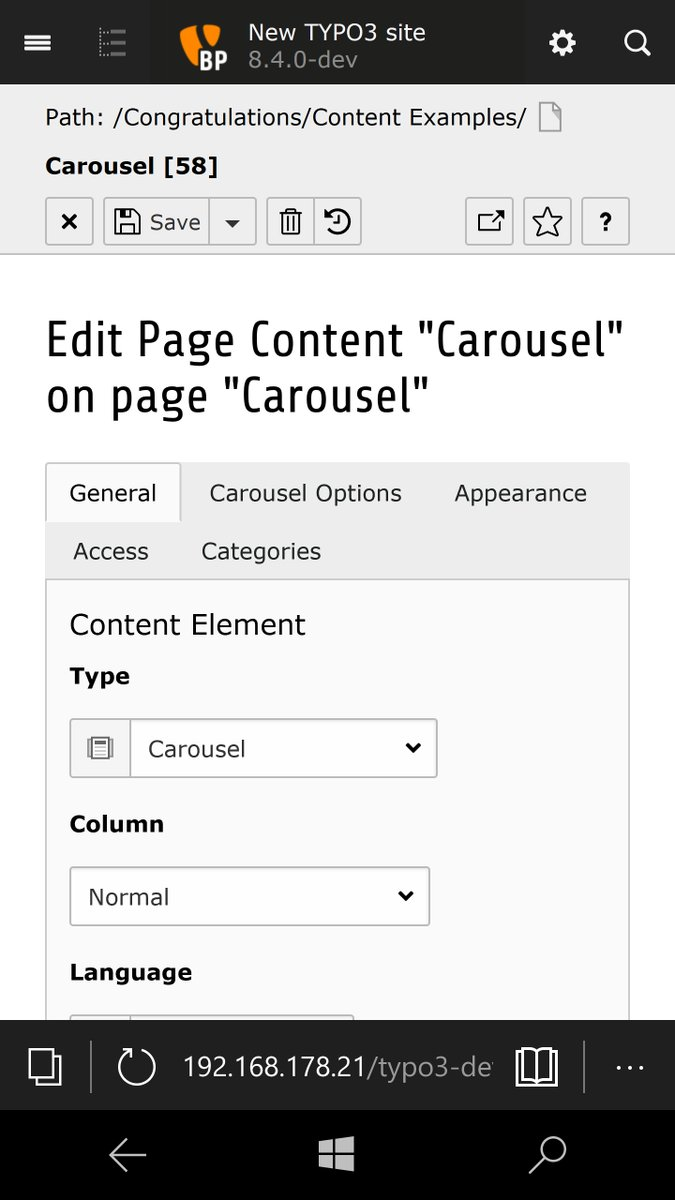
\includegraphics[width=0.25\linewidth]{BackendUserInterface/mobile-responsive-backend.jpg}
	\end{figure}

\end{frame}

% ------------------------------------------------------------------------------
% LTXE-SLIDE-START
% LTXE-SLIDE-UID:		664d708c-8791c332-a0b21119-89e9b1af
% LTXE-SLIDE-ORIGIN:	f6668b2d-8932a470-5b9c024c-e4e9f53a English
% LTXE-SLIDE-TITLE:		Install Tool: Upgrade Analysis
% ------------------------------------------------------------------------------

\begin{frame}[fragile]
	\frametitle{Gebruikersinterface backend}
	\framesubtitle{Installatie-module: Upgrade-analyse}

% The install tool, which is also a heavily used feature during updates between
% TYPO3 versions, has received some more beauty, basically finding all documented
% changes with a cool filter to show what is relevant for an integrator,
% extension author or site owner. Although this is already pretty cool, stay
% tuned for even better features to make migrations even easier between TYPO3
% versions!
% The migration and deprecation of existing options and switching within the TCA
% definitions we have in place since TYPO3 v7, is also visible in the Install Tool
% now.

	Upgrades van TYPO3 worden makkelijker met de nieuwe \textbf{Upgrade-analyse}-tool
	in de Installatie-module waar je gedocumenteerde wijzigingen tussen versies kunt vinden en filteren.

	\begin{figure}
		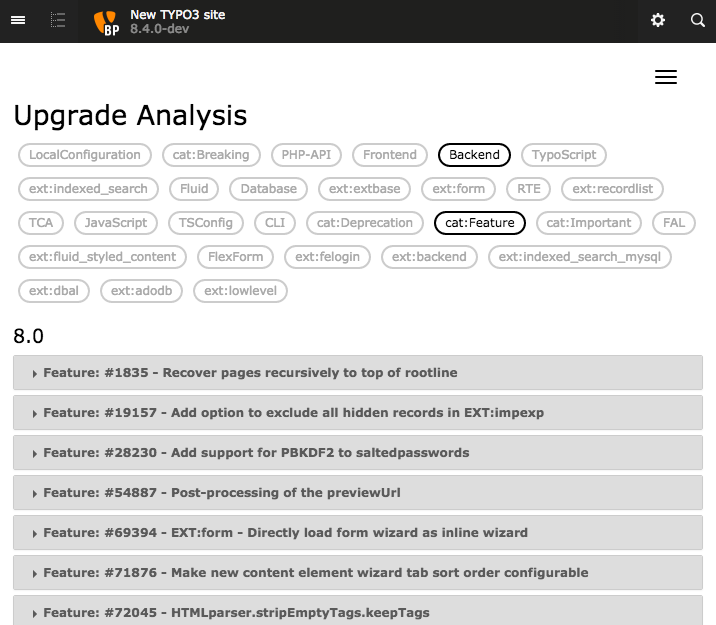
\includegraphics[width=0.45\linewidth]{BackendUserInterface/install-tool-upgrade-analysis.png}
	\end{figure}

\end{frame}

% ------------------------------------------------------------------------------
% LTXE-SLIDE-START
% LTXE-SLIDE-UID:		d5eab4e5-031c3ec2-6f3d3609-471c1e5b
% LTXE-SLIDE-ORIGIN:	9702aaf4-f02bbc35-67902b2e-42855506 English
% LTXE-SLIDE-TITLE:		Install Tool: Upgrade Analysis
% LTXE-SLIDE-REFERENCE:	#78222: Dump Class Loading Information UI in Install Tool
% ------------------------------------------------------------------------------

\begin{frame}[fragile]
	\frametitle{Gebruikersinterface backend}
	\framesubtitle{Installatie-module: Dump autoload-informatie}

	Aan de Installatie-module is een nieuwe actie toegevoegd om autoload-informatie te dumpen:
	informatie over de automatisch geladen klassen wordt dan opnieuw gegenereerd.

	\begin{figure}
		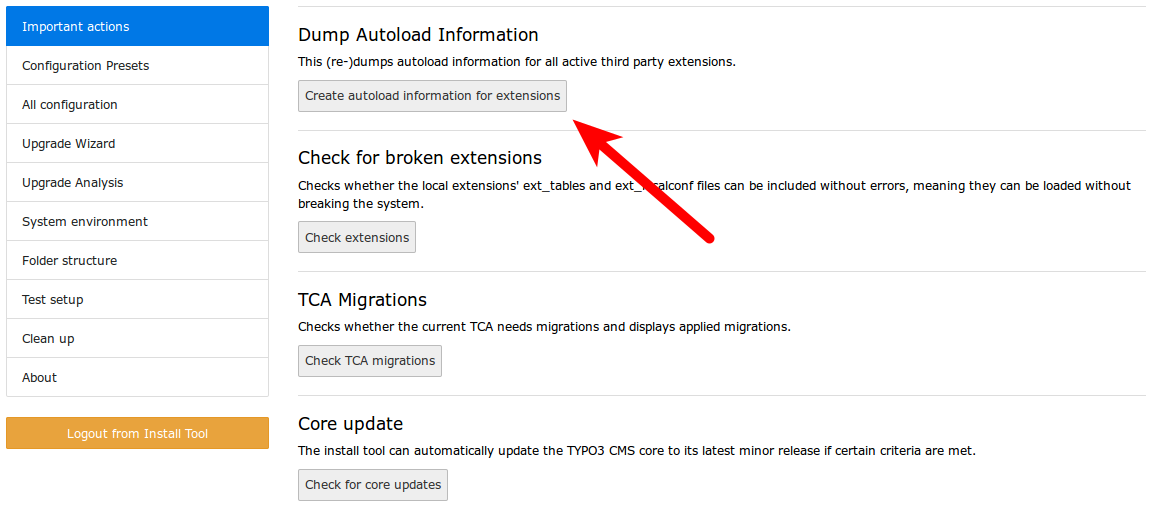
\includegraphics[width=0.8\linewidth]{BackendUserInterface/78222.png}
	\end{figure}

\end{frame}

% ------------------------------------------------------------------------------
% LTXE-SLIDE-START
% LTXE-SLIDE-UID:		2b4e8271-2a5cc903-ea1c1455-8d00dfaa
% LTXE-SLIDE-ORIGIN:	5a194e82-8eac7f1b-ef2730da-61d781b2 English
% LTXE-SLIDE-TITLE:		Install Tool: TCA Migration Messages
% LTXE-SLIDE-REFERENCE:	#77799: Display TCA migration messages in Install Tool
% ------------------------------------------------------------------------------

\begin{frame}[fragile]
	\frametitle{Gebruikersinterface backend}
	\framesubtitle{Installatie-module: Berichten over TCA-migraties}

	In de Installatie-module kunnen nu berichten over migraties van de TCA worden gecontroleerd.

	\begin{figure}
		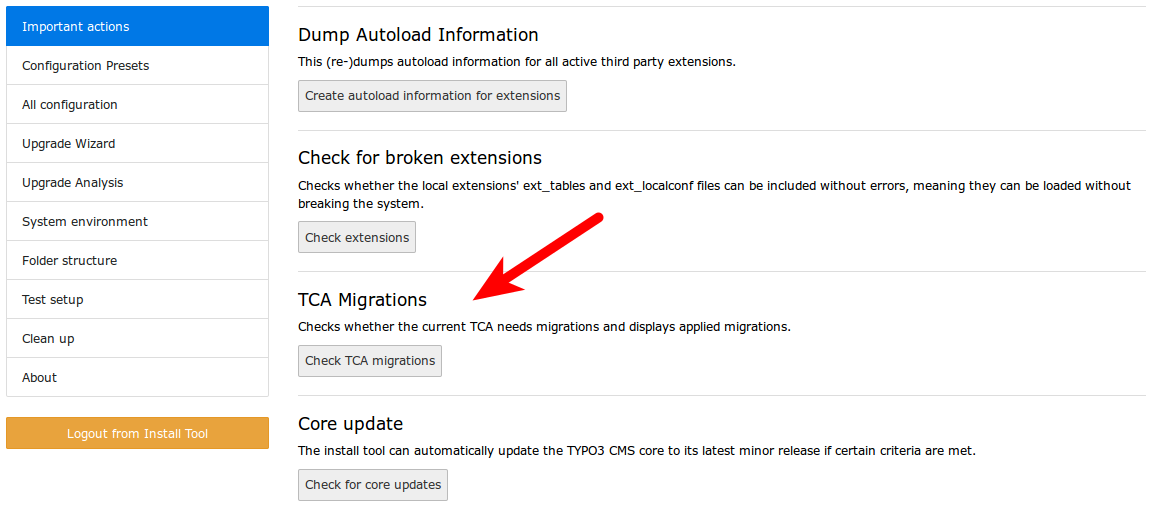
\includegraphics[width=0.8\linewidth]{BackendUserInterface/77799.png}
	\end{figure}

\end{frame}

% ------------------------------------------------------------------------------
% LTXE-SLIDE-START
% LTXE-SLIDE-UID:		90c017a4-984d55bd-ed745f9a-57c5c75d
% LTXE-SLIDE-ORIGIN:	1e11eae3-872938ec-9612c092-444c408a English
% LTXE-SLIDE-TITLE:		sys_language records are sortable now
% LTXE-SLIDE-REFERENCE:	#77652: Make sys_language records sortable
% ------------------------------------------------------------------------------

\begin{frame}[fragile]
	\frametitle{Gebruikersinterface backend}
	\framesubtitle{\texttt{sys\_language}-records}

	Voor extra gebruiksgemak kunnen \texttt{sys\_language}-records gesorteerd worden.

	\begin{figure}
		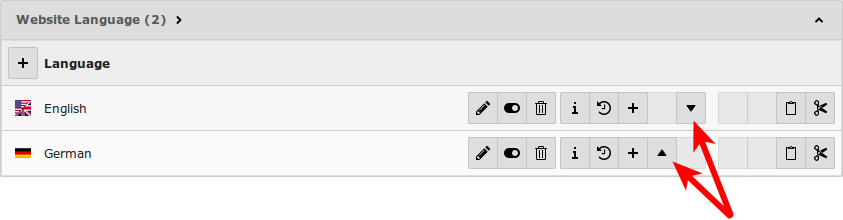
\includegraphics[width=0.8\linewidth]{BackendUserInterface/77652.png}
	\end{figure}

\end{frame}

% ------------------------------------------------------------------------------
% LTXE-SLIDE-START
% LTXE-SLIDE-UID:		0b1e8726-92a8c79e-24924c22-c1b73de2
% LTXE-SLIDE-ORIGIN:	a82823ff-94b9520f-5e6d6056-95f1a797 English
% LTXE-SLIDE-TITLE:		#77668: Hide table listing below group element
% ------------------------------------------------------------------------------

\begin{frame}[fragile]
	\frametitle{Gebruikersinterface backend}
	\framesubtitle{Lijst met tabellen onder groepselementen}

	\begin{itemize}

		\item De TCA-configuratieoptie \texttt{disable\_controls} van type "group"
			heeft nu een nieuwe instelling: \texttt{allowedTables}. Daarmee kunnen de hints 
			over de in het groepselement toegestane tabellen worden verborgen.

	\end{itemize}

	\begin{figure}
		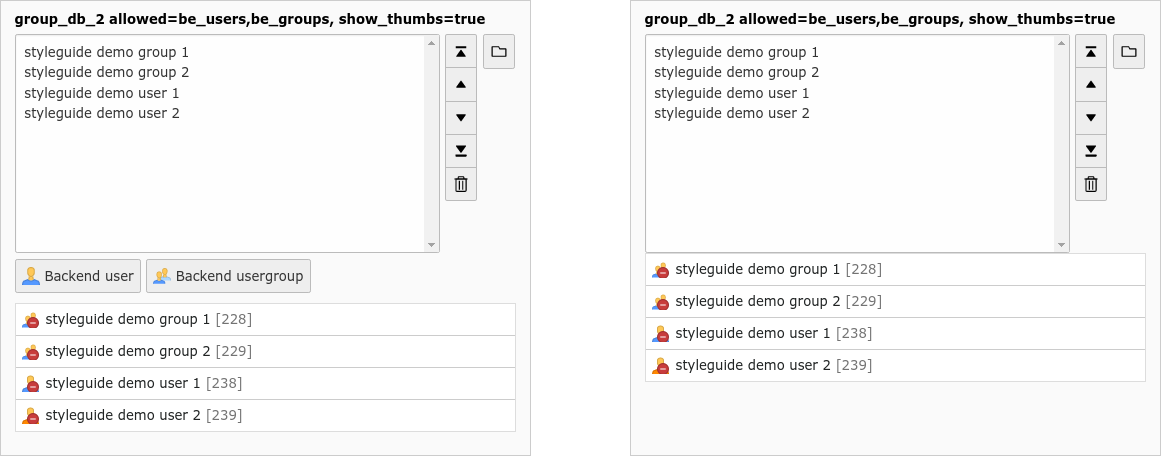
\includegraphics[width=0.85\linewidth]{BackendUserInterface/77668.png}
	\end{figure}

\end{frame}

% ------------------------------------------------------------------------------
